\documentclass{beamer}

% Preamble
\usepackage[latin1]{inputenc}
\usetheme{Warsaw}

% Title page
\title[Git - Version Control System]{Introduction  to Version Control with Git}
\author{Andreas Skielboe}
\institute{Dark Cosmology Centre \\ Niels Bohr Institute}
\date{\today}

% Settings
\def \figureHeight {130px}

\begin{document}

\begin{frame}
	\titlepage
\end{frame}

\begin{frame}{License}
	All images adapted from {\bf Pro Git} by Scott Chacon and released under license Creative Commons BY-NC-SA 3.0.
	\vskip15pt
	See \url{http://progit.org/}
\end{frame}

\begin{frame}{Why Use Version Control?}
	A Version Control System (VCS) is an integrated fool-proof framework for
	\begin{itemize}
		\item Backup and Restore
		\item Short and long-term undo
		\item Tracking changes
		\item Synchronization
		\item Collaborating
		\item Sandboxing
	\end{itemize}
	... with minimal overhead.
\end{frame}

\begin{frame}{Local Version Control Systems}
	Conventional version control systems provides some of these features by making a local database with all changes made to files.
	\begin{figure}
		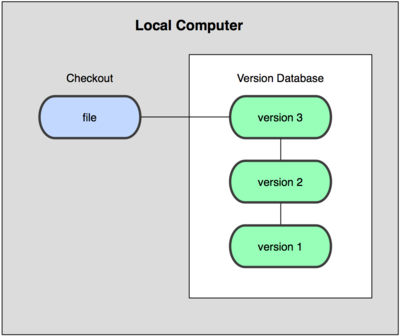
\includegraphics[height=\figureHeight]{images/local-version-control.png}
	\end{figure}
	Any file can be recreated by getting changes from the database and patch them up.
\end{frame}

\begin{frame}{Centralized Version Control Systems}
	To enable synchronization and collaborative features the database is stored on a central VCS server, where everyone works in the same database.
	\begin{figure}
		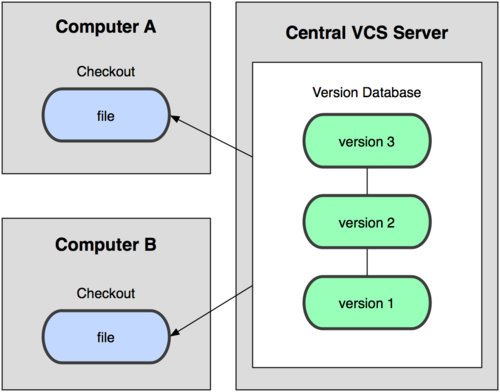
\includegraphics[height=\figureHeight]{images/central-version-control.png}
	\end{figure}
	Introduces problems: single point of failure, inability to work offline.
\end{frame}

\begin{frame}{Distributed Version Control Systems}
	To overcome problems related to centralization, distributed VCSs (DVCSs) were invented. Keeping a complete copy of database in every working directory.
	\begin{figure}
		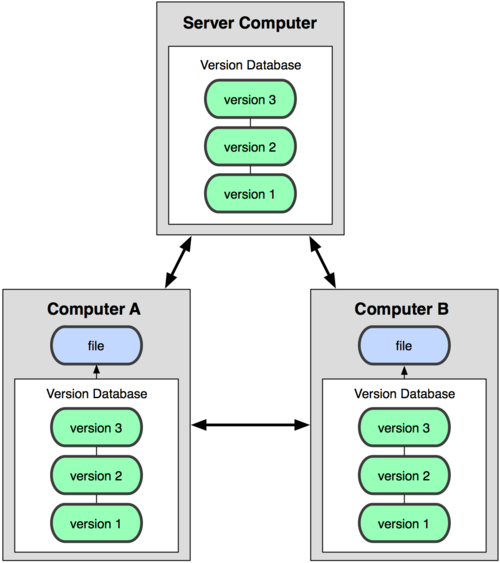
\includegraphics[height=\figureHeight]{images/distributed-version-control.png}
	\end{figure}
	Actually the most {\bf simple} and most {\bf powerful} implementation of any VCS.
\end{frame}

% % % Git Basics % % %
\begin{frame}{Git Basics}
	\begin{center}
		Git Basics
	\end{center}
\end{frame}

\begin{frame}{Git Basics - The Git Workflow}
	The simplest use of Git:
	\begin{itemize}
		\item {\bf Modify} files in your \emph{working directory}.
		\item {\bf Stage} the files, adding snapshots of them to your \emph{staging area}.
		\item {\bf Commit}, takes files in the staging area and stores that snapshot permanently to your \emph{Git directory}.
	\end{itemize}
\end{frame}

\begin{frame}{Git Basics - The Three States}
	The three basic states of files in your Git repository:
	\begin{figure}
		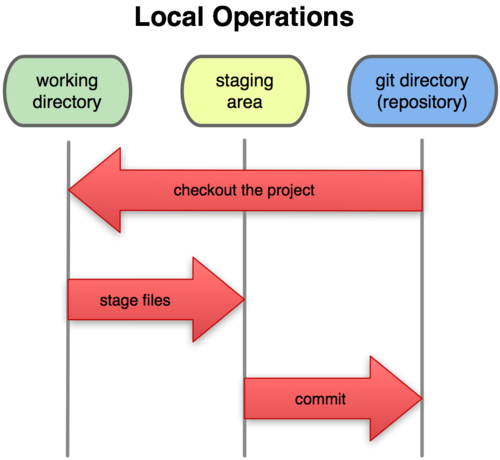
\includegraphics[height=\figureHeight]{images/the-three-states.png}
	\end{figure}
\end{frame}

\begin{frame}{Git Basics - Commits}
	Each commit in the git directory holds a snapshot of the files that were staged and thus went into that commit, along with author information.
	\begin{figure}
		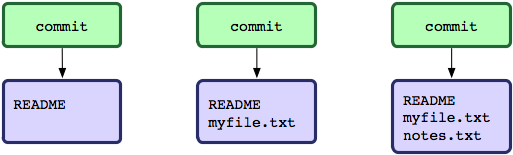
\includegraphics[]{images/commit-repository-data.png}
	\end{figure}
	Each and every commit can always be looked at and retrieved.
\end{frame}

\begin{frame}{Git Basics - File Status Lifecycle}
	Files in your working directory can be in four different states in relation to the current commit.
		\begin{figure}
		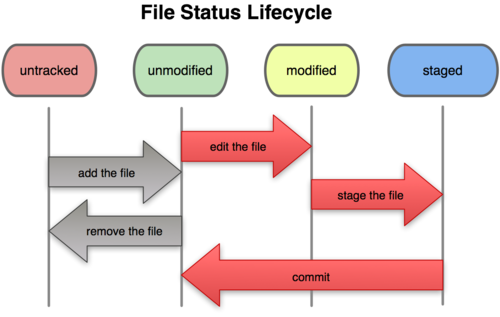
\includegraphics[height=\figureHeight]{images/file-status-lifecycle.png}
	\end{figure}
\end{frame}

\begin{frame}{Git Basics - Working with remotes}
	In Git {\bf all remotes are equal}.
	\vskip15pt
	A \emph{remote} in Git is nothing more than a link to another git directory.
\end{frame}

\begin{frame}{Git Basics - Working with remotes}
	The easiest commands to get started working with a remote are
	\begin{itemize}
		\item \emph{clone}: Cloning a remote will make a complete local copy.
		\item \emph{pull}: Getting changes from a remote.
		\item \emph{push}: Sending changes to a remote.
	\end{itemize}
	\vskip15pt
	Fear not! We are starting to get into more advanced topics. So lets look at some examples.
\end{frame}

\begin{frame}{Git Basics - Advantages}
	Basic advantages of using Git:
	\begin{itemize}
		\item Nearly every operation is local.
		\item Committed snapshots are always kept.
		\item Strong support for non-linear development.
	\end{itemize}
\end{frame}

\begin{frame}{Hands-on}
	\begin{center}
		Hands-on with Git \\ (here be examples)
	\end{center}
\end{frame}

\begin{frame}[fragile]{Hands-on - First-Time Git Setup}
	Before using Git for the first time:
	\begin{exampleblock}{Pick your identity}
		\begin{verbatim}
			$ git config --global user.name "John Doe"
			$ git config --global user.email johndoe@example.com
		\end{verbatim}
	\end{exampleblock}
	
	\begin{exampleblock}{Check your settings}
		\begin{verbatim}
			$ git config --list
		\end{verbatim}
	\end{exampleblock}
	
	\begin{exampleblock}{Get help}
		\begin{verbatim}
			$ git help <verb>
		\end{verbatim}
	\end{exampleblock}
\end{frame}

\begin{frame}[fragile]{Hands-on - Getting started with a bare remote server}
	Using a Git server (ie. no working directory / \emph{bare} repository) is the analogue to a regular centralized VCS in Git.
	\begin{figure}
		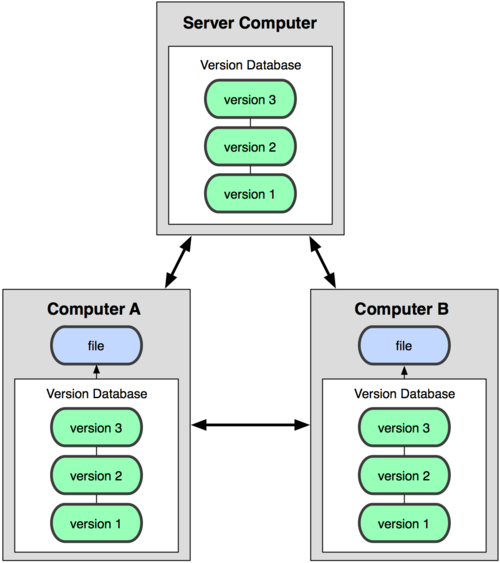
\includegraphics[height=\figureHeight]{images/distributed-version-control.png}
	\end{figure}
\end{frame}

\begin{frame}[fragile]{Hands-on - Getting started with remote server}
	When the remote server is set up with an initialized Git directory you can simply \emph{clone} the repository:
	\begin{exampleblock}{Cloning a remote repository}
		\begin{verbatim}
			$ git clone <repository>
		\end{verbatim}
	\end{exampleblock}
	You will then get a complete local copy of that repository, which you can edit.
\end{frame}

\begin{frame}[fragile]{Hands-on - Getting started with remote server}
	With your local working copy you can make any changes to the files in your working directory as you like. When satisfied with your changes you add any modified or new files to the staging area using \emph{add}:
	\begin{exampleblock}{Adding files to the staging area}
		\begin{verbatim}
			$ git add <filepattern>
		\end{verbatim}
	\end{exampleblock}
\end{frame}

\begin{frame}[fragile]{Hands-on - Getting started with remote server}
	Finally to commit the files in the staging area you run \emph{commit} supplying a \emph{commit message}.
	\begin{exampleblock}{Committing staging area to the repository}
		\begin{verbatim}
			$ git commit -m <msg>
		\end{verbatim}
	\end{exampleblock}
	Note that so far {\bf everything is happening locally} in your working directory.
\end{frame}

\begin{frame}[fragile]{Hands-on - Getting started with remote server}
	To {\bf share your commits} with the remote you invoke the \emph{push} command:
	\begin{exampleblock}{Pushing local commits to the remote}
		\begin{verbatim}
			$ git push
		\end{verbatim}
	\end{exampleblock}
	\vskip5pt
	To recieve changes that other people have pushed to the remote server you can use the \emph{pull} command:
	\begin{exampleblock}{Pulling remote commits to the local working directory}
		\begin{verbatim}
			$ git pull
		\end{verbatim}
	\end{exampleblock}
	\vskip5pt
	\begin{center}
		And {\bf thats it}.
	\end{center}
\end{frame}

\begin{frame}[fragile]{Hands-on - Summary}
	Summary of a minimal Git workflow:
	\begin{itemize}
		\item \verb+clone+ remote repository
		\item \verb+add+ you changes to the staging area
		\item \verb+commit+ those changes to the git directory
		\item \verb+push+ your changes to the remote repository
		\vskip15pt
		\item \verb+pull+ remote changes to your local working directory
	\end{itemize}
\end{frame}

\begin{frame}[fragile]{Checkout these slides}
	The \LaTeX-source of these slides is freely available on GitHub.
	\begin{exampleblock}{GitHub}
		\begin{footnotesize} \begin{verbatim}
			$ git clone git://github.com/askielboe/into-to-git-slides.git
		\end{verbatim} \end{footnotesize}
	\end{exampleblock}
	\vskip45pt
	\begin{center}
		Have fun using Git!
	\end{center}
\end{frame}

\begin{frame}[fragile]{References}
	Some good Git sources for information:
	\begin{itemize}
		\item Git Community Book - \url{http://book.git-scm.com/}
		\item Pro Git - \url{http://progit.org/}	
		\item Git Reference - \url{http://gitref.org/}
		\item GitHub - \url{http://github.com/}
		\item Git from the bottom up - \url{http://ftp.newartisans.com/pub/git.from.bottom.up.pdf}
		\item Understanding Git Conceptually - \url{http://www.eecs.harvard.edu/~cduan/technical/git/}
		\item Git Immersion - \url{http://gitimmersion.com/}
	\end{itemize}
\end{frame}

\end{document}